% -------------------------------------------------------------------------------------------------
%      MDSG Latex Framework
%      ============================================================================================
%      File:                  introduction-[UTF8,ISO8859-1].tex
%      Author(s):             Michael Duerr
%      Version:               1
%      Creation Date:         30. Mai 2010
%      Creation Date:         30. Mai 2010
%
%      Notes:                 - Example chapter
% -------------------------------------------------------------------------------------------------
%
\chapter{Related Work}\label{sec:RelatedWork}
- Definition of field of research \\
- Scientific Scope \\
- Which comparable work in research exists? \\
- Separation from other works

\section{Reinforcement Learning}
%https://lilianweng.github.io/lil-log/2018/02/19/a-long-peek-into-reinforcement-learning.html#key-concepts
\marginpar{rl components}
Sutton and Barto wrote in ``Reinforcement learning: An introduction''\cite{suba18} that Reinforcement learning (RL) is based on two components that interact with each other: an environment and an agent, see Figure \ref{fig:rl_cycle}. Those interactions take part during a time period with discrete time steps $t\in\mathbb{N}_0$ until a goal is reached or the ending condition applies. Formally the journey of the agent finding the goal state is described as the Markov Decision Process (MDP) and every method that leads the agent there is a reinforcement learning method. When multiple agents act in the same environment the Markov decision process is called a stochastic game \cite{buba10}.
% Initially the agent gets a starting environment state $S_0$, and can processes it to choose and execute an action $A_0$. This concludes the first time step. The environment changes based on the action and transitions into the next state $S_{1}$. In return the the agent receives the new state with a reward $R_{1}$ rating the action $A_0$. Afterwards the agent proceeds to execute actions which leads to the displayed cycle of Figure \ref{fig:rl_cycle}.
\begin{figure}[hpbt]
    \centering
    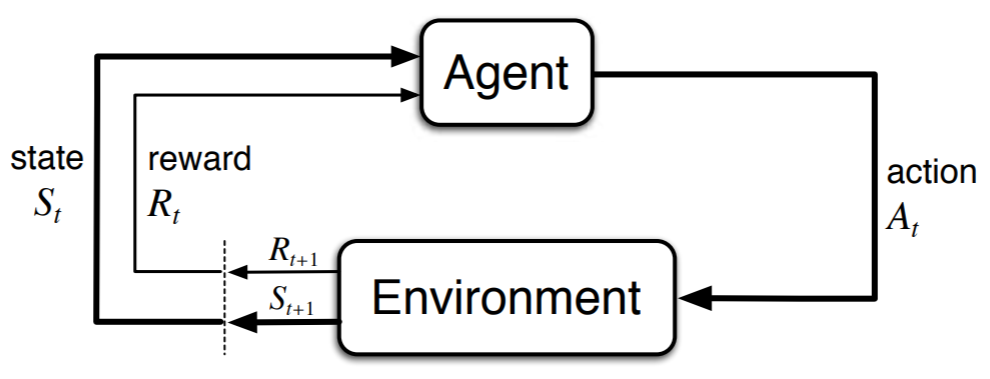
\includegraphics[width=0.6\textwidth]{pictures/RLInteractionSB}\\
    \caption[reinforcement learning cycle]{The cycle of agent-environment interaction as
        shown in ``Reinforcement learning: An introduction''\cite{suba18}}\label{fig:rl_cycle}
\end{figure}

\marginpar{sets and values}
The state $S_t$ is part of a set $S$ containing all possible environment states. Since its likely that not all actions are valid in each environment state the agents action selection is based on a restricted set $A_t\in A(S_t)$. In a multiagent environment however, every agent chooses its action and adds it into a joint action set, which is executed collectively on the environment \cite{buba10}. The reward $R_t$ is element of a set of possible rewards $R$, which is a subset of real numbers $R \subset \mathbb{R}$. Therefore, the reward can potentially be negative or very low to emphasize a bad action. The general concept of RL, as defined by Sutton and Barto, is to maximize rewards. Thus, unlike machine learning approaches the agent starts with no knowledge about good or bad actions and enhances the decision-making by aiming to improve the reward.

\marginpar{policy}
Sutton and Barto continue by defining the agents action selection with respect to the current state as a policy $\pi$. They explain further that a policy could be as simple as a lookup table, mapping states to actions or it could contain a complicated search process for the best decision. In most cases it is of stochastic nature, mapping actions and states with probabilities. During environment interactions agents gain rewards, which then can be used to update the policy accordingly. For example, should the reward be low or negative it could be interpreted as a penalty. In return the policy $\pi(a \mid s)$ could then be adapted to set a very low probability for that action in combination with that certain state. So next time the agent finds itself in that state the bad action is not very likely to be chosen again.

\marginpar{value function}
While rewards only rate the immediate situation, a value function, i.e. the state-value function $v_{\pi}(s)$ for a policy $\pi$ can be used to estimate the long-term value of a state $s$. The result is the total accumulated reward an agent could get down the line following that state and choosing actions based on the current policy. States that offer immediate high reward could end in
% The value function is of importance, due to states bringing high rewards could end in
low reward streaks. Or the opposite could be the case, where a low reward state could subsequently yield high rewards. Therefore, value functions are of great use to achieve the maximum reward.
% Other value functions can also take the executed
% action into account to reach the state from which the rewards are estimated.

\marginpar{exploration vs exploitation}
The last part to note about RL is that it entails the problem of balancing exploration and exploitation. In order to learn, an agent has to explore the options given. However, since maximizing rewards is the goal an agent could become greedy and exploit its knowledge by choosing actions of which it knows to result in small but positive rewards. If an agent doesn't explore enough the best action sequence will stay hidden and if an agent always explores without exploiting its knowledge, chances are that the reward will not be optimal.

\section{Credit Assignment Problem}
\marginpar{intro and comp. problems}
Realistic RL scenarios often involve multiple agents solving problems together, for example robots working in warehouses and factories. Such multiagent environments come with many difficulties. On the one hand in a scenario where agents work independently it is very probable that they get in each other's way in order to score highest or finish a task, preventing the overall goal to be achieved.

\marginpar{coop problems}
In cooperative environments on the other hand, agents share the reward and therefore can not tell who contributed useful actions and who did not. Hence, all agents receive the same reward regardless of their contribution, which aggravates learning. The independence problem is discussed in chapter \ref{market} whereas the cooperation challenge is the focus point of this chapter.

\marginpar{coop and problem}
Sutton and Barto \cite{suba18} define a RL environment as cooperative, when agents execute their actions collectively each time step but receive one overall reward in return. In this case individual learning is difficult or even impossible. Collective actions may contain bad choices that could be rewarded or, in case of a penalty,  good actions that would be punished. Deciding which agent deserves more or less reward, when splitting it up is referred to as the credit assignment problem (CAP) \cite{mi61}.

\marginpar{CAP definition and kinds}
The CAP originated in a one-agent environment that only returned reward once the goal is reached or the terminating condition applied. A popular example of this is a chess game. In 1961, Minsky \cite{mi61} elaborated on this by explaining that a player wins or loses the game, but cannot retrace which decision got him there. Sutton later on decomposed the CAP into subproblems, namely the structural and temporal CAP \cite{su84}. He suggests that the temporal CAP is assigning credit to each chess move, by determining when the position improves or worsen, rewarding or penalizing that certain action. On the contrary, the structural CAP is assigning credit to the internal decision that leads to each particular action.

\marginpar{CAP multi}
% Sutton also refers to a chess game to explain the subproblems. 
Transferring the single-agent CAP into a multiagent environment Agogino and Tumer \cite{agtu04} imply that the problem shifts from being of temporal to structural manner. They explain that while a single agent faces the temporal CAP due to many steps taken within an extended time period, in the multiagent case it becomes a structural CAP because of multiple actions in a single-time-step. Since the actions are executed all at once, the problem is now to evaluate the decision that lies underneath.
% They explain that a single agent faces the temporal CAP when many steps are taken within an extended time period so learning from the returned reward at the end is problematic. Whereas in the multiagent setting it becomes a structural CAP because of multiple actions leading to a shared reward during a single-time-step.

\marginpar{cap solution dr}
Over the years many solutions and theories emerged in order to solve various CAP scenarios. An example for a simple approach is the difference reward (DR) \cite{agtu04},\cite{ngku18}. The idea is to calculate the reward with the joint multiagent actions as always. In every step however, each agent decomposes that reward by calculating the difference between a new reward and the old one. The new reward is generated with the same actions, only modifying the action of the current agent, setting it to a default or waiting value. With this method each agent has the opportunity to learn how they contributed to the resulting state and reward, enabling individual learning. High DR values indicate lucrative actions of the analyzing agent. The opposite case applies for low valued DRs.

\section{Markets}\label{market}
\marginpar{markets and advantage}
\marginpar{sm}
\marginpar{am}
\marginpar{what is expected?}